\section{实验总体方案}
本系统的测试分为两个部分, 第一部分是功能测试, 第二部分是性能测试\juhao 功能测试部分主要测试监控应用启动, 监控Java方法调动, 监控本地函数执行以及脱壳功能是否正常运行, 结果是否准确; 性能测试部分主要测试在监控系统运行时的性能开销, 并同Android Device Monitor做对比测试\juhao 
\section{实验运行环境}
由于本系统基于Android8.1构建, 并运行于真机上, 因此本次实验会涉及两台设备\juhao 设备1是用于配置和控制本系统的个人电脑, 设备2是运行该系统的智能手机, 两台设备的硬件和软件环境如表\ref{environment}所示\juhao

\begin{table}[ht]
	\centering
	\caption{实验设备环境}
	\resizebox{\textwidth}{!}{%
		\begin{tabular}{lllll}
			\hline
			设备                               & 型号                       & \textbf{CPU(型号/主频)}           & \textbf{内存} & 操作系统         \\ \hline
			\multicolumn{1}{c}{\textbf{设备1}} & Lenovo XiaoXin 700-15ISK & Intel core i5 6300HQ / 2.3GHZ & 8GB         & 深度操作系统15.9.3 \\ \hline
			\textbf{设备2}                     & Google Nexus 5X          & MSM8992 / 1.8GHZ              & 2GB         & Android8.1   \\ \hline
		\end{tabular}%
	}
	\label{environment}
\end{table}
\section{功能测试}
本次功能测试使用了支付宝应用的10.1.62版本(应用软件包名com.eg.android.\\AlipayGphone)本文作者开发的一款名为noticer的应用(应用软件包名top.january147\\.noticer)来进行\juhao noticer应用经过360加固保\upcite{360jiagubao}加固, 以检测本系统功能的有效性\juhao 
\subsection{监控应用启动功能测试}
在设备1上开启终端, 输入adb logcat|grep EvMonitor等待读取本系统监控应用启动的记录\juhao 然后执行如下操作:在设备2上启动支付宝应用, 然后退出支付宝应用再启动noticer应用\juhao

从终端中读取的监控记录如图\ref{testAppStart1}所示\juhao
\begin{figure}[ht]
	\centering
	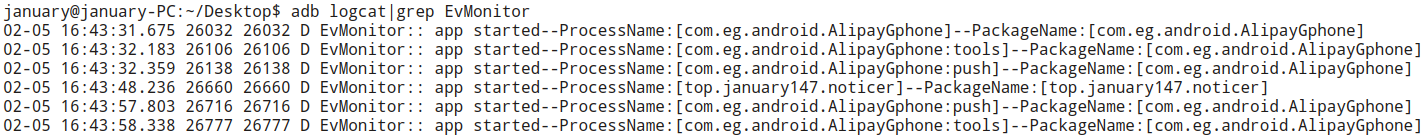
\includegraphics[width=\textwidth]{test_app_start_1.png}
	\caption{应用启动监控记录}
	\label{testAppStart1}
\end{figure}
监控记录显示支付宝应用的首先启动, 该应用共计启动了3个进程, 进程名分别为com.eg.android.AlipayGphone\dunhao com.eg.a-ndroid.AlipayGphone:push\dunhao 和com.eg.android.AlipayGphone:tools; 接着记录了noticer的启动, 该应用只启动了一个进程, 进程名为top.january147.noticer; 后边又记录了支付宝启动的两个进程,com.eg.android.AlipayGphone:tools和com.eg.android.A-lipayGphone:push而测试流程中并没有再次执行支付宝, 可以看到支付宝有自动启动的行为\juhao 

\subsection{监控Java方法调用功能测试}
\label{testJavacallA}
在设备1上开启终端, 键入adb shell进入设备2的shell\juhao 此时利用setprop命令设置系统属性em.target\_app为noticer软件的包名top.january147.noticer, 然后再执行logcat | grep Evmonitor查看系统运行情况\juhao 在设备2上启动noticer, 启动后界面如图\ref{testNoticer}所示, 点击底部的电话通知服务按钮启动电话通知服务, 等待启动完成再次点击该按钮关闭电话通知服务, 完成后退出应用\juhao 此时在设备1上运行脚本pull\_log\_dir.sh获取目标应用日志文件夹\juhao
\begin{figure}[ht]
	\centering
	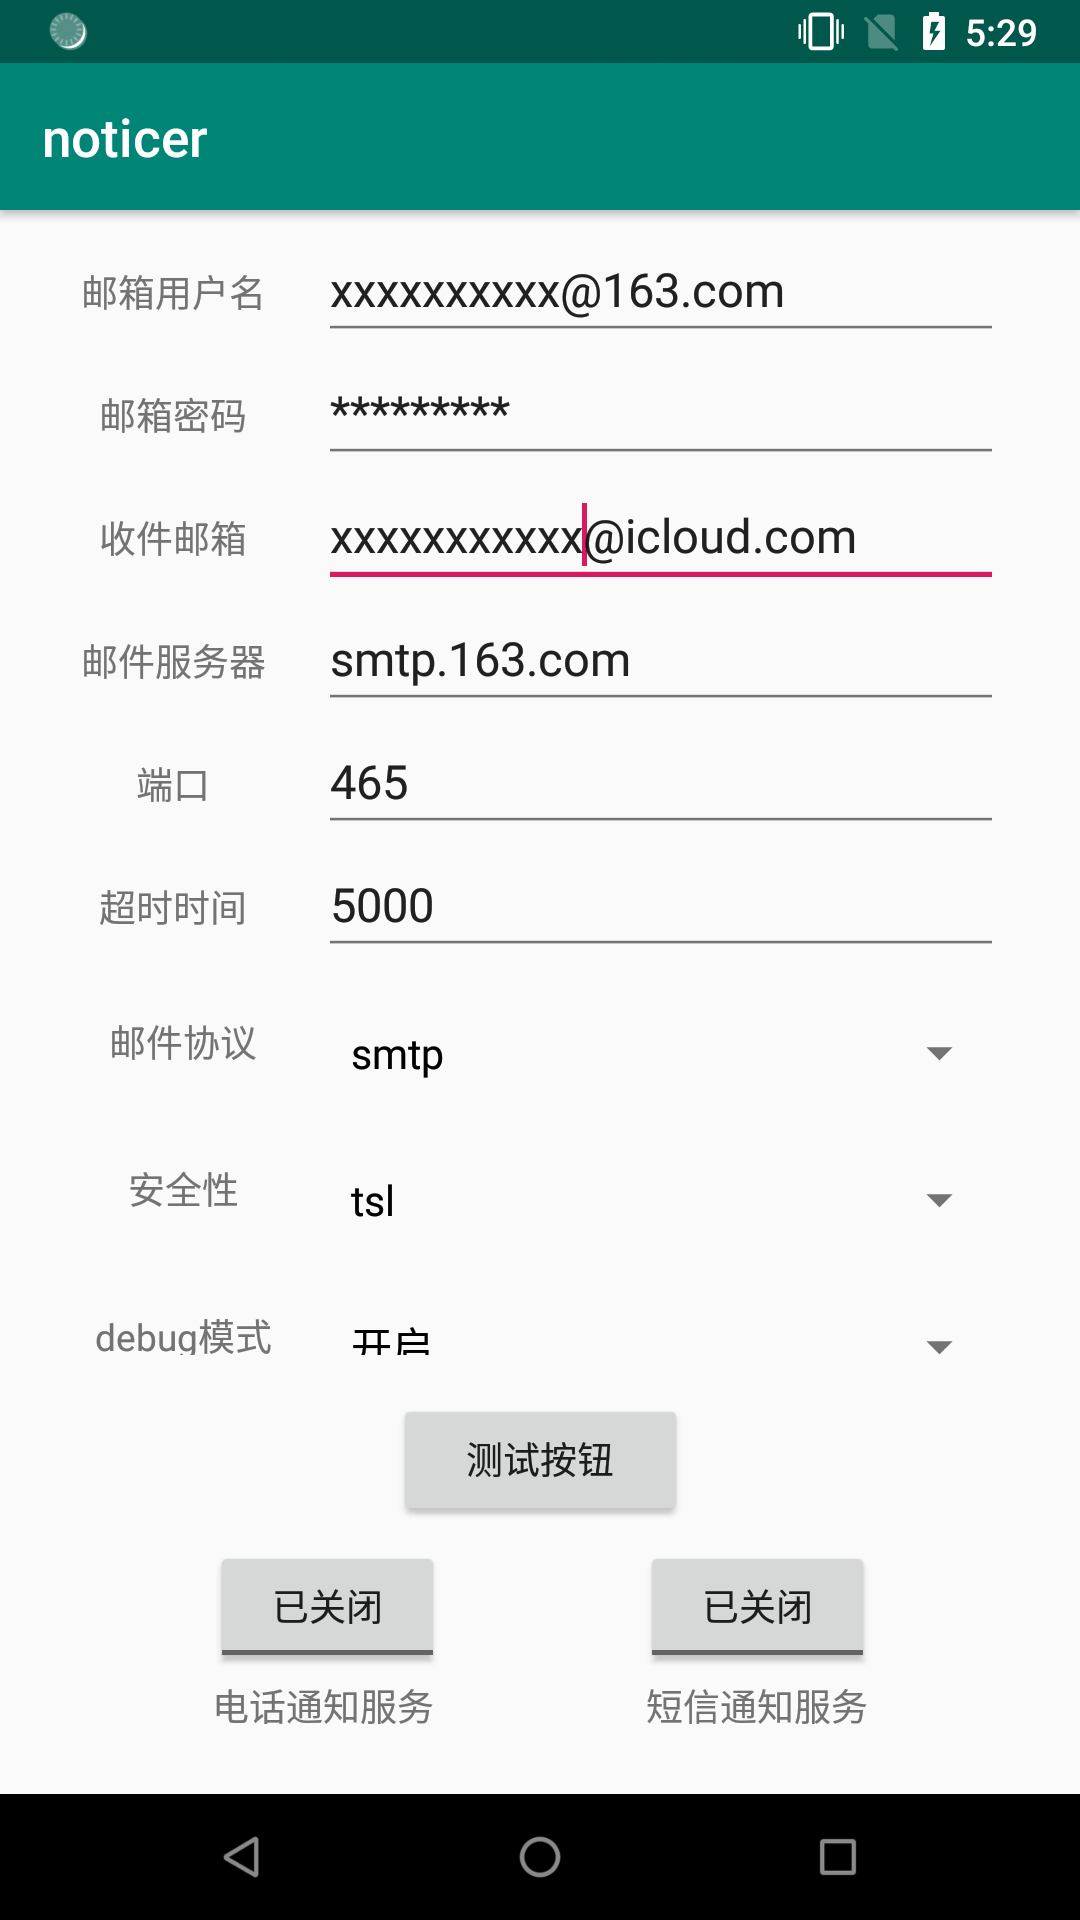
\includegraphics[width=4cm]{test_noticer.png}
	\caption{noticer界面}
	\label{testNoticer}
\end{figure}

图\ref{testJavacall}是终端中显示的本系统的运行信息\juhao 可以看到, 应用启动监控模块检测到目标应用启动后调用本地层的接口进行了一系列初始化操作, 包括创建日志文件夹, 分配日志缓冲区等等, 此外还记录了dex文件解析的情况\juhao 
\begin{figure}[ht]
	\centering
	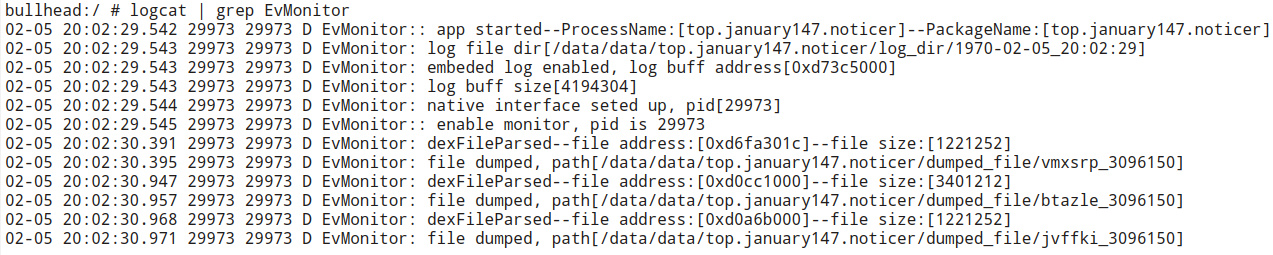
\includegraphics[width=\textwidth]{test_javacall.png}
	\caption{监控系统运行日志}
	\label{testJavacall}
\end{figure}

打开脚本pull\_log\_dir.sh从目标应用目录下取得的日志文件夹会发现一个以时间命名的文件夹, 该文件夹记录了应用在上述执行过程中的日志数据, 其文件如图\ref{testLogFile}所示\juhao 可以看到有许多em\_开头后接数字编号编号的log文件, 编号即为log文件生成的顺序, 这些文件记录了应用在上述过程执行中全部Java方法调用\juhao 
\begin{figure}[ht]
	\centering
	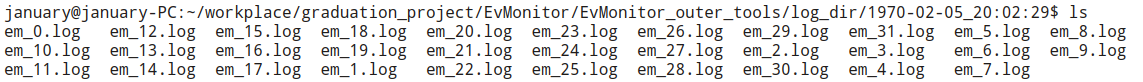
\includegraphics[width=\textwidth]{test_log_file.png}
	\caption{Java调用记录日志文件}
	\label{testLogFile}
\end{figure}

限于论文篇幅原因, 本文使用脚本log\_filter.sh过滤上述日志文件, 生成只包含noticer自身方法调用的记录文件, 并在其中搜索关于执行应用运行时两次点击按钮的调用记录, 结果如图\ref{testServiceStart}和\ref{testServiceStop}所示\juhao 由于启动服务需要进行许多初始化操作, 流程较长图\ref{testServiceStart}是服务启动开始时和完成时的部分调用记录\juhao 图\ref{testServiceStart}是关闭服务的完整调用记录\juhao 每条记录的格式为"线程号 执行方式 方法名称", 执行方式由两个大写字母和"--"组成, 第一个字母为I表示方法开始执行, 为O表示方法执行结束; 第二个字母为V表示通过ArtMethod::Invoke函数执行, 为E表示通过Execute函数执行\juhao 
\begin{figure}[ht]
	\centering
	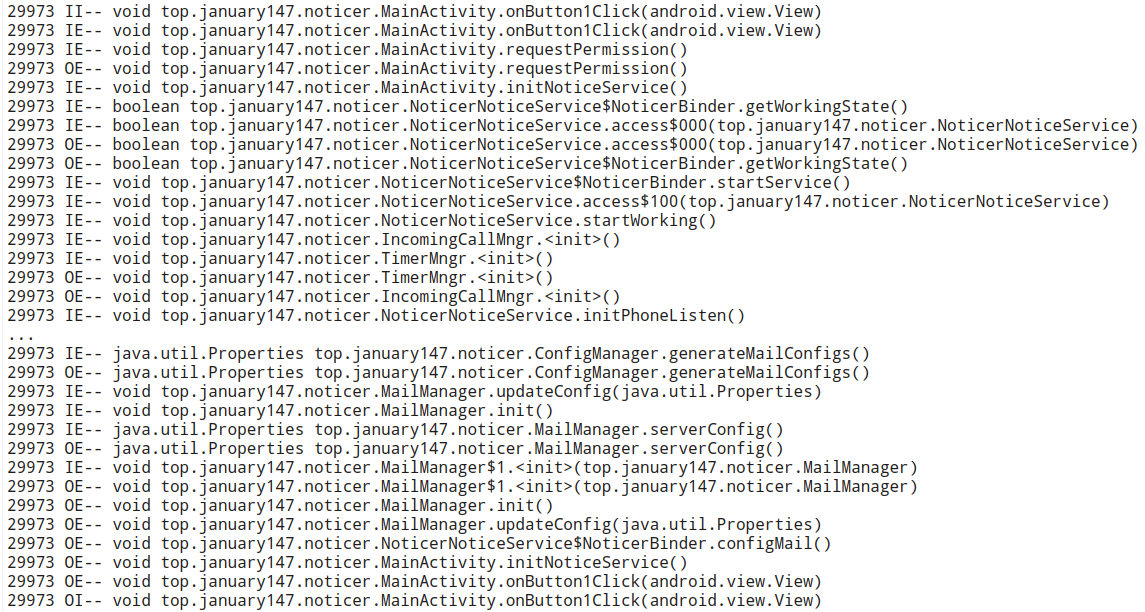
\includegraphics[width=\textwidth]{test_service_start.png}
	\caption{启动电话通知服务的调用记录}
	\label{testServiceStart}
\end{figure}
\begin{figure}[ht]
	\centering
	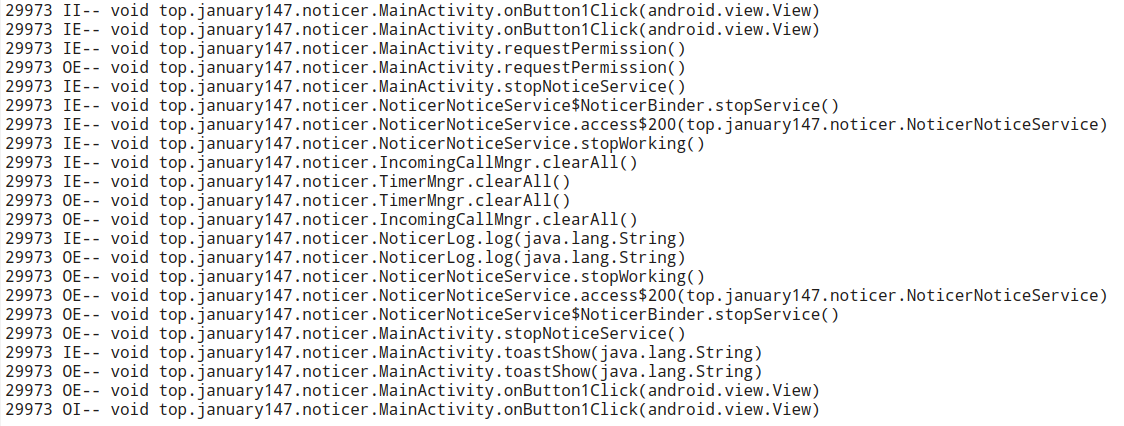
\includegraphics[width=\textwidth]{test_service_stop.png}
	\caption{关闭电话通知服务的调用记录}
	\label{testServiceStop}
\end{figure}

\subsection{脱壳功能测试}
\ref{testJavacallA}小节测试流程中本系统已经启动并执行了脱壳功能, 在本小节的测试中直接使用脚本pull\_dumped\_file.sh从目标应用文件夹获取得到包含dex文件的文件夹\juhao 该文件夹中为3个dex文件, 使用dex2jar工具转换成jar文件后文件夹内容如图\ref{testDexFile}所示\juhao 没有后缀名的3个文件为脱壳工具抓取的dex文件, 其他3个为dex2jar工具转换后对应的jar文件\juhao 
\begin{figure}[ht]
	\centering
	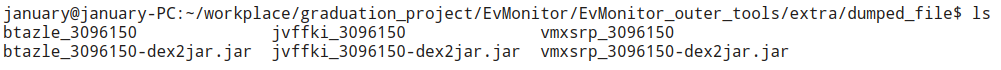
\includegraphics[width=\textwidth]{test_dex_file.png}
	\caption{脱壳工具抓取的dex文件}
	\label{testDexFile}
\end{figure}

使用jd-gui打开3个jar文件后成功在名为btazle\_3096150-dex2jar.jar的文件中找到了实现应用真实功能的类, 成功实现了脱壳\juhao 图\ref{testOrgClass}是jd-gui工具查看的结果, top.january147.noticer包下的类即为应用本身的类, 右侧显示的为\ref{testJavacallA}小节中Java方法调用记录中的onButton1Click方法源代码\juhao 
\begin{figure}[ht]
	\centering
	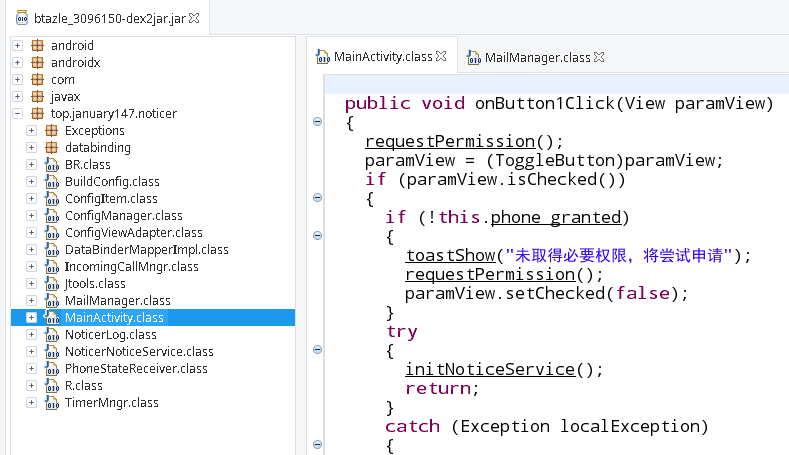
\includegraphics[width=\textwidth]{test_org_class.png}
	\caption{脱壳后得到应用本身的类}
	\label{testOrgClass}
\end{figure}

\subsection{监控本地函数调用功能测试}
开启监控目标应用noticer, 本系统记录的本地调用信息会保存到应用目录下的log\_dir文件夹中, 从中获取的本地函数调用信息如图\ref{testNativeCall}所示\juhao 
\begin{figure}[ht]
	\centering
	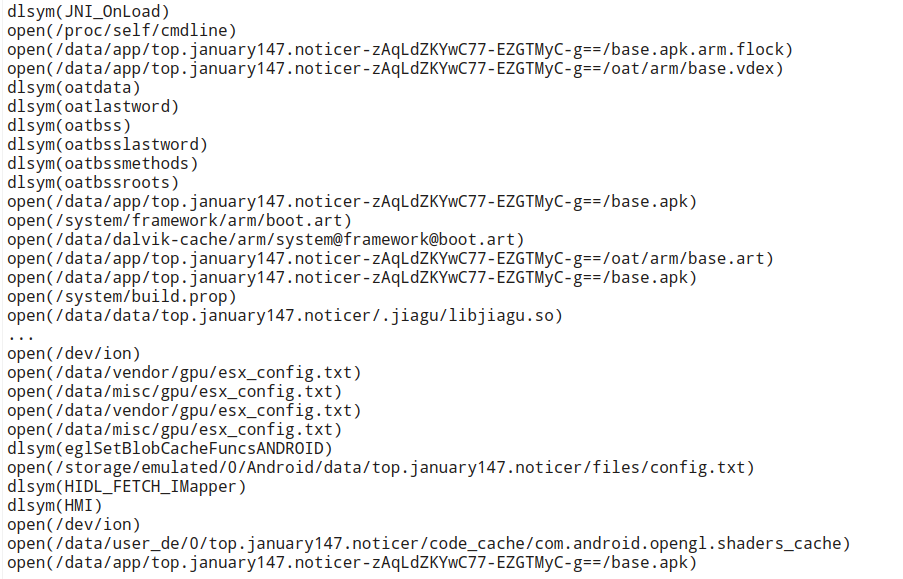
\includegraphics[width=\textwidth]{test_native_call.png}
	\caption{本地函数调用记录}
	\label{testNativeCall}
\end{figure}

\section{性能测试}
由于本系统的主要性能开销在于记录方法调用时的性能开销, 针对cpu性能的性能测试工具无法成功检测本系统的性能, 因此本文开发了一个简单的测试Java方法调用性能检测的应用, 该应用将一个简单的无内部调用的java方法执行固定次数并测量总用时用于评价Java方法调用性能\juhao 本文使用了该应用对本系统和Android Device Monitor的Method Profile功能进行了测试, 结果如图\ref{testOverhead}所示\juhao 
\begin{figure}[ht]
	\centering
	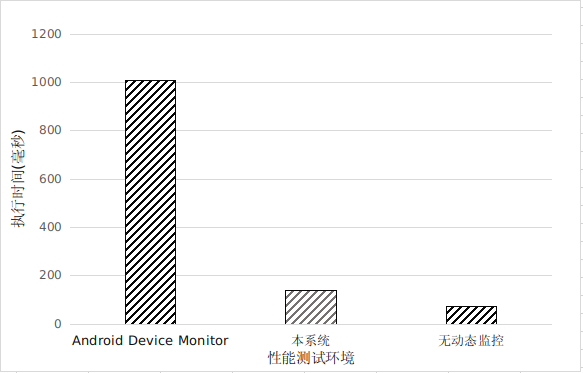
\includegraphics[width=8cm]{test_overhead.png}
	\caption{本地函数调用记录}
	\label{testOverhead}
\end{figure}
其中的执行时间为10次测量结果取平均值得到的\juhao

\section{结果分析}
功能测试的结果显示本系统的基本功能正常, 能够实现对应用启动\dunhao Java方法调用\dunhao 本地函数调用的监控和以及脱壳功能, 系统设计原理可行\juhao 性能测试的结果显示本系统的执行耗时约为正常执行时的两倍, 而Android Device Monitor执行耗时约为正常执行的14倍, 本系统为Android Device Monitor的Method Profile功能运行效率的7倍, 因此十分高效\juhao 

